\documentclass[a4paper,12pt]{article}
\usepackage[utf8]{inputenc}
\usepackage{graphicx}
\usepackage{graphics}
\usepackage{hyperref}
\usepackage{geometry}
\usepackage{pdflscape}
\usepackage{caption}

\usepackage[spanish]{babel}
\graphicspath{ {build/} } 
\geometry{left=2cm, right=2cm, top=2cm, bottom=2cm}

\begin{document}

\begin{titlepage}
    \begin{center}
        \vspace*{3cm}
        
        {\Huge \textbf{Laboratorio 1 - Grupo 7}}\\[1cm]
        {\LARGE Panel solar automático:\\ [0.5cm]Planificación y Gestión del Proyecto}\\[2cm]
        
        \vfill
        
        {\Large \textbf{Integrantes}}\\[.5cm]
        \large
        \begin{tabular}{c c}
            Gartner, Francisco Nehuen & 69864/6 \\
            Marchesotti, Guido Daniel & 69923/9 \\
            Rosa, Fausto Pablo & 69843/1 \\
        \end{tabular}
        
        \vspace{1cm}
        
        \begin{figure}[b]
            \centering
            
\includegraphics[width=1\linewidth]{LOGOSFI-UNLP-color-01.png}
        \end{figure}
        
    \end{center}
\end{titlepage}

\newpage
\section{Ciclo de vida}

Con el objetivo de desarrollar un sistema de seguimiento solar automático, se plantea una planificación estructurada pero flexible, basada en un enfoque de ciclo de vida híbrido. Esta metodología permitirá definir con claridad los objetivos desde el inicio, manteniendo a su vez la capacidad de adaptación frente a eventualidades que puedan surgir durante el desarrollo. Si bien se busca cumplir con un cronograma establecido, se contempla una cierta elasticidad en los plazos para acomodar ajustes o mejoras necesarias.

\section{Organización del equipo de trabajo}
El equipo de trabajo se organizará mediante un esquema rotativo de tareas, lo cual permite que todos los integrantes participen activamente en cada una de las etapas del proyecto. Esta dinámica favorece la adquisición de experiencia integral y fortalece el trabajo colaborativo, al mismo tiempo que permite repartir la carga laboral de manera equitativa. Cada miembro tendrá la posibilidad de involucrarse tanto en el diseño como en la implementación y prueba del sistema.

\section{Cronograma y desglose de actividades}
El cronograma tentativo, ilustrado en la Figura \ref{cronograma}, distribuye las actividades a lo largo de varias semanas, permitiendo visualizar los tiempos asignados a cada fase y facilitar el seguimiento del avance.
Como se observa en el gráfico, se prevé que las etapas de planificación inicial tardarán alrededor de 4 a 5 semanas, siendo estas junto con las de desarrollo de software las etapas más extensas y de mayor importancia, fundamentales para el correcto desarrollo del proyecto. Las etapas de software y maquetas se llevarán a cabo en paralelo, permitiendo flexibilidad en términos de plazos de ejecución. El responsable de cada etapa estará indicado en el siguiente desglose de cronograma\\

\begin{itemize}
    \item Primera etapa de planificación (Gartner): Durante la primera etapa se prevé realizar un análisis inicial completo que incluirá la definición del propósito del sistema, la identificación de los materiales necesarios, la estimación preliminar de costos y la elaboración de un cronograma general. También se abordará la recopilación de información técnica, y se procederá a una distribución inicial de tareas.
    \item Segunda etapa de planificación (Marchesotti): A continuación, se trabajará en la elaboración de esquemas y diagramas del sistema, abarcando tanto el diseño mecánico como el eléctrico. Esta instancia servirá como base para tomar decisiones informadas respecto a los componentes a adquirir. Entre los elementos previstos se encuentran sensores, un panel solar, motores para orientación, un microcontrolador, un sistema de transmisión de datos y una fuente de alimentación adecuada. Además, será necesario desarrollar un soporte estructural que asegure la estabilidad y movilidad del panel.
    \item Obtención de insumos (Rosa).
    \item Desarrollo de software de etapa temprana (Gartner): Testeo y programacion de sensores y actuadores.
    \item Realización de maquetas y prototipos (Marchesotti):se llevarán a cabo a partir de maquetas y prototipos funcionales, que permitirán verificar el comportamiento del sistema en condiciones controladas.
    \item Acondicionamiento y etapa de pruebas (Rosa): Pruebas preliminares que verifiquen el comportamiento funcional del proyecto, cumpliendo con objetivos básicos del proyecto. 
    \item Etapa alfa (Gartner): En esta instancia se someterá al sistema a distintas condiciones de iluminación y orientación, será clave para ajustar parámetros, depurar el software y evaluar el desempeño general.
    \item Puesta a punto y modificaciones finales (Marchesotti): se llevaran a cabo las modificaciones finales antes de la entrega del proyecto terminado.
    \item Entrega del proyecto final
\end{itemize}

\section{Adquisiciones y Presupuesto}
En cuanto al presupuesto, se ha estimado un costo total cercano a los \hyperref[tabla]{\$150.000}, Este monto abarca tanto los elementos electrónicos como los materiales de construcción y montaje. A su vez, contempla posibles modificaciones. Se procurará reutilizar componentes disponibles y optar por soluciones accesibles sin comprometer la funcionalidad del sistema.\\

\begin{table}[h!]
        \centering
        \begin{tabular}{|l|c|}
            \hline
            Concepto  & Costo Estimado \\ 
            \hline
            Sensores & \$20.000 \\
            Panel solar  & \$23.000 \\
            Motores  & \$25.000 \\
            Soporte pivote & \$8.000 \\
            Microcontrolador  & \$10.000 \\
            Sistema de comunicación  & \$12.000 \\
            Sistema de Alimentación  & \$50.000 \\
            \hline
            \textbf{Total Estimado} & \$148.000 \\
            \hline
        \end{tabular}
        \captionof{figure}{Tabla con precios aproximados consultados al momento de realizar el informe }
        \label{tabla}
        
    \end{table}


\newpage
\begin{landscape}
    \thispagestyle{empty} % quita número de página si molesta
    \begin{center}
        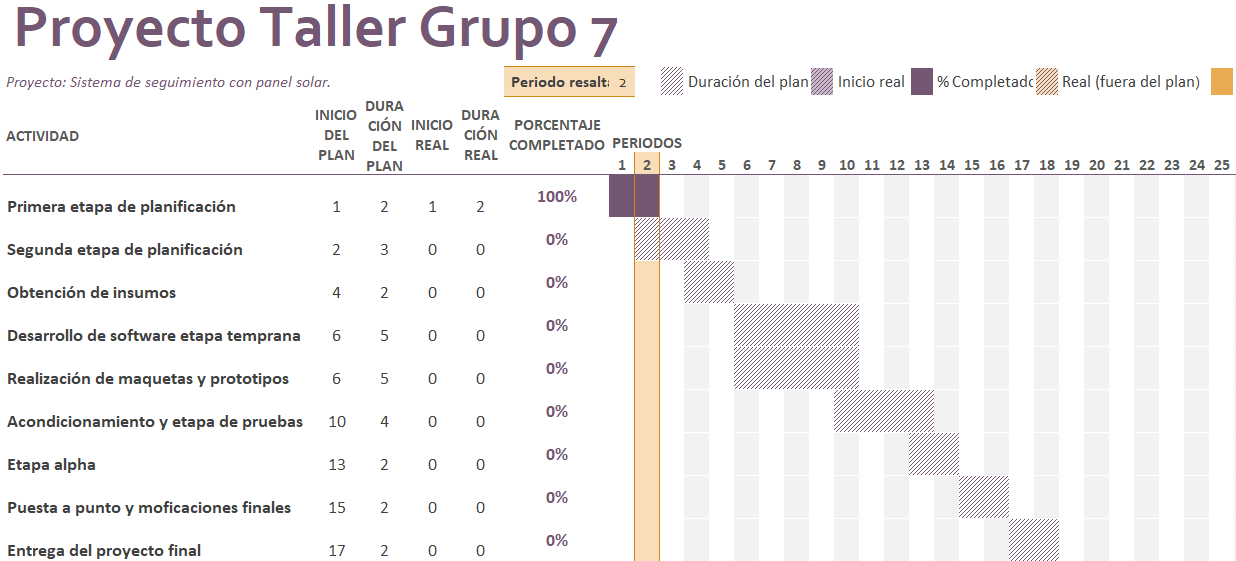
\includegraphics[width=0.95\linewidth]{grantt-V3.png}
        \captionof{figure}{Cronograma en semanas}
        \label{cronograma}
    \end{center}
    En la figura se puede observar varias columnas con los tiempos estimados para cada actividad junto con los valores reales que efectivamente tardo la misma. Usando los tiempos reales se va completando la columna de 'Porcentaje completado'. Para un mejor seguimiento visual del cronograma, se implementa un indicador del 'Periodo resaltado'
\end{landscape}
\end{document}
